\documentclass[12pt,a4paper]{report}

% ─── Packages ────────────────────────────────────────────────────────────────
\usepackage[utf8]{inputenc}
\usepackage[T1]{fontenc}
\usepackage{geometry}
\usepackage{graphicx}
\usepackage{xcolor}
\usepackage{hyperref}
\usepackage{fancyhdr}
\usepackage{titlesec}
\usepackage{tocloft}
\usepackage{enumitem}
\usepackage{booktabs}
\usepackage{array}
\usepackage{longtable}
\usepackage{tabularx}
\usepackage{float}
\usepackage{amsmath}
\usepackage{amssymb}
\usepackage{setspace}
\usepackage{parskip}
\usepackage{mdframed}
\usepackage{tikz}
\usepackage{pgf-umlcd}
\usepackage{listings}
\usepackage{caption}
\usepackage{subcaption}
\usepackage{afterpage}

% ─── Geometry ────────────────────────────────────────────────────────────────
\geometry{
  top=2.5cm, bottom=2.5cm,
  left=3cm,  right=2.5cm,
  headheight=15pt
}

% ─── Colors ──────────────────────────────────────────────────────────────────
\definecolor{darkplum}{HTML}{4F0C28}
\definecolor{periwinkle}{HTML}{C5D2F8}
\definecolor{offwhite}{HTML}{F1FAEE}
\definecolor{gris}{HTML}{555555}
\definecolor{lightgray}{HTML}{F5F5F5}
\definecolor{codegreen}{HTML}{2E7D32}
\definecolor{codegray}{HTML}{757575}

% ─── Hyperref ────────────────────────────────────────────────────────────────
\hypersetup{
  colorlinks=true,
  linkcolor=darkplum,
  urlcolor=darkplum,
  citecolor=darkplum,
  pdftitle={Rapport PFA – ManageraHub},
  pdfauthor={Aya Raji Allah, Adam Tchich}
}

% ─── Chapter / Section Styles ────────────────────────────────────────────────
\titleformat{\chapter}[display]
  {\normalfont\huge\bfseries\color{darkplum}}
  {\chaptertitlename\ \thechapter}{20pt}{\Huge}
\titlespacing*{\chapter}{0pt}{30pt}{40pt}

\titleformat{\section}
  {\normalfont\Large\bfseries\color{darkplum}}
  {\thesection}{1em}{}

\titleformat{\subsection}
  {\normalfont\large\bfseries\color{gris}}
  {\thesubsection}{1em}{}

\titleformat{\subsubsection}
  {\normalfont\normalsize\bfseries\color{gris}}
  {\thesubsubsection}{1em}{}

% ─── Header / Footer ─────────────────────────────────────────────────────────
\pagestyle{fancy}
\fancyhf{}
\fancyhead[L]{\small\textcolor{darkplum}{\textbf{ManageraHub}} – Rapport PFA}
\fancyhead[R]{\small\textcolor{gris}{\leftmark}}
\fancyfoot[C]{\thepage}
\renewcommand{\headrulewidth}{0.4pt}
\renewcommand{\headrule}{\hbox to\headwidth{\color{darkplum}\leaders\hrule height \headrulewidth\hfill}}

% ─── Line spacing ────────────────────────────────────────────────────────────
\setstretch{1.3}

% ─── Custom box ──────────────────────────────────────────────────────────────
\newmdenv[
  linecolor=darkplum,
  linewidth=1.5pt,
  backgroundcolor=offwhite,
  leftmargin=0, rightmargin=0,
  innerleftmargin=10pt, innerrightmargin=10pt,
  innertopmargin=8pt, innerbottommargin=8pt,
  roundcorner=4pt
]{infobox}

% ─── Listings (code) ─────────────────────────────────────────────────────────
\lstset{
  basicstyle=\ttfamily\small,
  keywordstyle=\color{darkplum}\bfseries,
  commentstyle=\color{codegreen},
  stringstyle=\color{codegray},
  backgroundcolor=\color{lightgray},
  frame=single, framerule=0.4pt,
  breaklines=true, numbers=left,
  numberstyle=\tiny\color{codegray}
}

% ═══════════════════════════════════════════════════════════════════════════════
\begin{document}

% ─── Page de garde ───────────────────────────────────────────────────────────
\begin{titlepage}
\centering
{\color{darkplum}\rule{\linewidth}{2pt}}\\[0.4cm]
{\Large\textbf{École Marocaine des Sciences de l'Ingénieur}}\\[0.1cm]
{\large EMSI -- Honoris United Universities}\\[0.1cm]
{\color{darkplum}\rule{\linewidth}{0.5pt}}\\[1cm]

{\large Module~: \textbf{Projet de Fin d'Année (PFA)} -- 3IIR16}\\[1.5cm]

{\color{darkplum}\rule{0.8\linewidth}{1pt}}\\[0.4cm]
{\Huge\bfseries\color{darkplum} RAPPORT DE PROJET}\\[0.3cm]
{\LARGE\bfseries Plateforme de Recrutement}\\[0.2cm]
{\huge\bfseries\color{darkplum} ManageraHub}\\[0.4cm]
{\color{darkplum}\rule{0.8\linewidth}{1pt}}\\[2cm]

\begin{tabular}{rl}
\textbf{Réalisé par :} & Aya RAJI ALLAH \\[0.2cm]
                       & Adam TCHICH \\[0.8cm]
\textbf{Filière :}     & Ingénierie Informatique et Réseaux (3IIR16) \\[0.2cm]
\textbf{Encadrant :}   & \textit{(Nom de l'encadrant)} \\[0.8cm]
\textbf{Année universitaire :} & 2025/2026
\end{tabular}

\vfill
{\color{darkplum}\rule{\linewidth}{2pt}}
\end{titlepage}

% ─── Remerciements ───────────────────────────────────────────────────────────
\chapter*{Remerciements}
\addcontentsline{toc}{chapter}{Remerciements}
\thispagestyle{plain}

Nous tenons tout d'abord à exprimer notre profonde gratitude envers notre encadrant pédagogique pour sa disponibilité, ses précieux conseils et son soutien constant tout au long de la réalisation de ce projet. Ses orientations éclairées nous ont permis d'avancer avec méthode et rigueur.

Nos remerciements vont également à l'ensemble du corps enseignant de l'École Marocaine des Sciences de l'Ingénieur (EMSI) qui, par leurs enseignements de qualité et leurs encouragements, nous ont fourni les bases théoriques et pratiques indispensables à l'élaboration de ce travail.

Nous remercions sincèrement nos familles et proches pour leur soutien moral indéfectible et leurs encouragements tout au long de notre parcours académique. Leur présence et leur bienveillance ont été une source inestimable de motivation.

Enfin, nos remerciements s'adressent à tous ceux qui, de près ou de loin, ont contribué à la réussite de ce projet de fin d'année, qu'il s'agisse de camarades de promotion, de professionnels du secteur ou de toute autre personne ayant partagé ses connaissances et son expérience.

\vspace{1cm}
\begin{flushright}
\textit{Aya RAJI ALLAH \& Adam TCHICH}\\
\textit{Année universitaire 2025/2026}
\end{flushright}

% ─── Résumé (français) ───────────────────────────────────────────────────────
\chapter*{Résumé}
\addcontentsline{toc}{chapter}{Résumé}
\thispagestyle{plain}

\begin{infobox}
\textbf{Mots-clés :} Plateforme de recrutement, Django, MySQL, Python, Gestion des candidatures, Interface web, Offres d'emploi.
\end{infobox}

\vspace{0.5cm}

Dans un contexte marqué par une transformation numérique accélérée et une concurrence croissante sur le marché de l'emploi, la mise en place de solutions digitales efficaces pour faciliter le recrutement est devenue une nécessité incontournable. Ce rapport présente le projet de fin d'année intitulé \textbf{ManageraHub}, une plateforme web de recrutement développée dans le cadre du module PFA de la filière 3IIR16 à l'EMSI.

ManageraHub est une application web full-stack conçue pour mettre en relation les candidats à la recherche d'opportunités professionnelles avec les entreprises souhaitant recruter des profils qualifiés. La plateforme offre un espace dédié à chaque type d'acteur~: les candidats peuvent y créer leur profil, consulter et filtrer les offres d'emploi, postuler en ligne en joignant leur CV et lettre de motivation, et suivre en temps réel le statut de leurs candidatures. Les entreprises, quant à elles, disposent d'un tableau de bord complet leur permettant de publier et gérer leurs offres, de consulter les profils des candidats et de prendre des décisions de recrutement éclairées.

Le développement de ManageraHub s'appuie sur le framework \textbf{Django} (Python) pour la partie backend, couplé à \textbf{MySQL} comme système de gestion de base de données relationnelle. L'interface utilisateur a été conçue selon des principes d'ergonomie modernes, en mettant l'accent sur la clarté, la simplicité et la fluidité de navigation. Un module d'administration permet en outre de superviser l'ensemble des activités de la plateforme.

Ce document présente successivement le contexte et les objectifs du projet, la conception détaillée du système à travers différents diagrammes UML, et enfin les perspectives d'évolution envisagées.

% ─── Abstract (anglais) ──────────────────────────────────────────────────────
\chapter*{Abstract}
\addcontentsline{toc}{chapter}{Abstract}
\thispagestyle{plain}

\begin{infobox}
\textbf{Keywords:} Recruitment platform, Django, MySQL, Python, Application management, Web interface, Job offers.
\end{infobox}

\vspace{0.5cm}

In a context characterized by accelerated digital transformation and increasing competition in the job market, implementing efficient digital solutions to facilitate recruitment has become an undeniable necessity. This report presents the end-of-year project entitled \textbf{ManageraHub}, a web-based recruitment platform developed as part of the PFA module in the 3IIR16 program at EMSI.

ManageraHub is a full-stack web application designed to connect job-seeking candidates with companies looking to recruit qualified profiles. The platform provides a dedicated space for each type of actor: candidates can create their profile, browse and filter job listings, apply online by submitting their CV and cover letter, and track the real-time status of their applications. Companies, on the other hand, benefit from a comprehensive dashboard that allows them to publish and manage job offers, review candidate profiles, and make informed recruitment decisions.

The development of ManageraHub relies on the \textbf{Django} framework (Python) for the backend, coupled with \textbf{MySQL} as the relational database management system. The user interface has been designed according to modern ergonomic principles, emphasizing clarity, simplicity, and smooth navigation. An administration module further enables supervision of all platform activities.

This document successively presents the project context and objectives, the detailed system design through various UML diagrams, and finally the envisaged future development perspectives.

% ─── Table des matières ──────────────────────────────────────────────────────
\tableofcontents
\thispagestyle{plain}

% ─── Liste des figures ───────────────────────────────────────────────────────
\listoffigures
\addcontentsline{toc}{chapter}{Liste des figures}

% ─── Liste des tableaux ──────────────────────────────────────────────────────
\listoftables
\addcontentsline{toc}{chapter}{Liste des tableaux}

% ─── Introduction générale ───────────────────────────────────────────────────
\chapter*{Introduction Générale}
\addcontentsline{toc}{chapter}{Introduction Générale}
\markboth{Introduction Générale}{}

L'essor des technologies de l'information et de la communication a profondément transformé les pratiques du recrutement. Là où les annonces d'emploi étaient autrefois publiées dans la presse papier et les candidatures envoyées par courrier postal, le numérique a redéfini l'ensemble du processus, le rendant plus rapide, plus accessible et plus interactif. Aujourd'hui, aussi bien les candidats que les recruteurs s'attendent à disposer d'outils performants, intuitifs et centralisés pour gérer l'ensemble du cycle de recrutement.

Malgré la présence de nombreuses plateformes généralistes sur le marché, comme LinkedIn, Indeed ou Rekrute, un besoin persiste pour des solutions plus ciblées, plus simples d'utilisation et mieux adaptées à des contextes spécifiques. Ces plateformes existantes sont souvent perçues comme complexes, surchargées de fonctionnalités et peu adaptées aux besoins des petites et moyennes entreprises ou des jeunes diplômés en début de carrière.

C'est dans ce contexte que s'inscrit le projet \textbf{ManageraHub}, une plateforme web de recrutement développée dans le cadre du module Projet de Fin d'Année (PFA) de la filière Ingénierie Informatique et Réseaux (3IIR16) à l'École Marocaine des Sciences de l'Ingénieur (EMSI). ManageraHub vise à proposer une solution centralisée, moderne et intuitive pour faciliter la mise en relation entre les candidats et les entreprises, en simplifiant le processus de dépôt de candidatures et de gestion du recrutement.

Ce rapport s'articule autour de trois chapitres principaux. Le \textbf{premier chapitre} présente le contexte général du projet, en exposant la problématique identifiée, les objectifs poursuivis, l'analyse des besoins fonctionnels et non fonctionnels, ainsi que les contraintes techniques encadrant le développement. Le \textbf{deuxième chapitre} est consacré à la conception du système, avec une présentation détaillée des différents diagrammes UML utilisés pour modéliser l'architecture et le comportement de la plateforme. Le \textbf{troisième chapitre} présente les réalisations concrètes de la plateforme à travers un aperçu des différentes interfaces développées, accompagné d'explications sur les fonctionnalités implémentées.

% ═══════════════════════════════════════════════════════════════════════════════
%  CHAPITRE 1 : CONTEXTE DU PROJET
% ═══════════════════════════════════════════════════════════════════════════════
\chapter{Contexte du Projet}

\section*{Introduction}
\addcontentsline{toc}{section}{Introduction}

Ce premier chapitre pose les fondations conceptuelles et organisationnelles du projet ManageraHub. Il vise à situer le projet dans son environnement, à définir clairement la problématique à laquelle il répond, et à identifier les différents acteurs impliqués. Une analyse approfondie des besoins fonctionnels et non fonctionnels permettra de délimiter avec précision le périmètre du système à développer, avant de présenter les critères d'acceptabilité retenus pour valider la solution.

% ─────────────────────────────────────────────────────────────────────────────
\section{Présentation du projet}

\subsection{Contexte général}

Avec l'évolution rapide du marché de l'emploi et l'accélération de la transformation numérique, les méthodes traditionnelles de recrutement ont cédé la place à des approches digitales plus efficaces et plus accessibles. Les entreprises cherchent aujourd'hui à optimiser leurs processus de sélection, à toucher un plus grand nombre de candidats qualifiés et à réduire les délais de recrutement. De leur côté, les candidats souhaitent disposer d'une visibilité complète sur les opportunités disponibles et d'un suivi transparent de leurs démarches.

Le projet \textbf{ManageraHub} naît de ce double constat. Il s'agit d'une plateforme web de recrutement conçue pour centraliser l'ensemble du processus, depuis la publication d'une offre d'emploi par une entreprise jusqu'à la décision finale concernant la candidature d'un profil. La plateforme se positionne comme un intermédiaire neutre et efficace, offrant à chaque acteur un espace adapté à ses besoins spécifiques.

\subsection{Présentation de ManageraHub}

ManageraHub est une application web full-stack développée avec le framework Django (Python), s'appuyant sur une base de données MySQL pour la persistance des données. La plateforme cible deux catégories principales d'utilisateurs~: les candidats en recherche d'emploi ou de stage, et les entreprises souhaitant recruter des profils adaptés à leurs besoins. Un troisième acteur, l'administrateur, assure la supervision et la maintenance générale du système.

La plateforme propose une interface claire et intuitive, respectant une charte graphique professionnelle articulée autour de la couleur principale Dark Plum (\texttt{\#4F0C28}), symbole de confiance et de professionnalisme. Les typographies Poppins et Inter ont été sélectionnées pour garantir une lisibilité optimale et renforcer le caractère moderne de l'interface.

\subsection{Objectifs du projet}

Le projet ManageraHub poursuit plusieurs objectifs complémentaires qui structurent l'ensemble du développement et guident les choix de conception retenus.

L'objectif principal est de \textbf{mettre en relation efficacement les candidats et les entreprises} en proposant un espace centralisé où l'ensemble du cycle de recrutement peut être géré de manière fluide et transparente. La plateforme cherche ainsi à réduire les frictions liées aux processus traditionnels, souvent fragmentés entre plusieurs outils et canaux de communication.

Sur le plan fonctionnel, ManageraHub vise à \textbf{permettre aux entreprises de publier et de gérer leurs offres d'emploi} de manière autonome, avec la possibilité de consulter les candidatures reçues et de prendre des décisions de recrutement documentées. Pour les candidats, la plateforme doit offrir un environnement complet permettant de \textbf{rechercher des offres, de postuler en ligne et de suivre l'évolution de chaque candidature} en temps réel.

Un objectif transversal porte sur la \textbf{qualité de l'expérience utilisateur}. L'interface doit être suffisamment simple pour être accessible à tous, y compris aux utilisateurs peu familiers avec les outils numériques, tout en étant suffisamment riche pour répondre aux besoins professionnels des recruteurs. Enfin, la \textbf{sécurité des données} constitue un objectif non négociable, dans un contexte où les informations personnelles des candidats et des entreprises doivent être protégées conformément aux bonnes pratiques de sécurité informatique.

% ─────────────────────────────────────────────────────────────────────────────
\section{Analyse des besoins}

\subsection{Problématique}

La problématique centrale du projet peut être formulée de la manière suivante~: comment concevoir et développer une plateforme web de recrutement qui soit à la fois fonctionnelle, ergonomique et sécurisée, capable de répondre simultanément aux attentes des candidats, des entreprises et des administrateurs, tout en se distinguant des solutions existantes par sa simplicité et sa clarté ?

Cette problématique soulève plusieurs défis techniques et fonctionnels. Il s'agit notamment de concevoir une architecture logicielle robuste permettant de gérer plusieurs types d'utilisateurs avec des droits et des interfaces différenciés, d'implémenter un système de gestion des candidatures capable de gérer les transitions d'état (en attente, accepté, refusé, entretien), et de garantir la sécurité des données sensibles échangées sur la plateforme.

\subsection{Besoins fonctionnels}

Les besoins fonctionnels représentent l'ensemble des fonctionnalités que la plateforme doit offrir à ses différents utilisateurs. Ils ont été identifiés à partir d'une analyse approfondie des processus de recrutement et des attentes exprimées par les cibles visées.

\subsubsection{Fonctionnalités communes à tous les utilisateurs}

Tout utilisateur de la plateforme doit pouvoir créer un compte, se connecter de manière sécurisée et se déconnecter. Le système doit proposer une gestion différenciée des profils selon le rôle attribué lors de l'inscription, garantissant ainsi que chaque acteur n'accède qu'aux fonctionnalités qui lui sont destinées. Une interface d'accueil publique doit également présenter les services de la plateforme aux visiteurs non encore inscrits.

\subsubsection{Fonctionnalités dédiées aux candidats}

Le candidat doit pouvoir créer un compte personnalisé et compléter son profil avec l'ensemble de ses informations personnelles et professionnelles. La plateforme doit lui permettre de téléverser son curriculum vitæ et d'y joindre une lettre de motivation personnalisée pour chaque candidature. Il doit également disposer d'un moteur de recherche et de filtrage des offres d'emploi selon des critères variés tels que le domaine d'activité, la ville ou le type de contrat. Une fois sa candidature soumise, le candidat doit pouvoir consulter l'historique de toutes ses démarches et suivre en temps réel l'évolution du statut de chacune d'elles.

\subsubsection{Fonctionnalités dédiées aux entreprises}

L'entreprise doit pouvoir créer un compte dédié et compléter son profil institutionnel. Elle dispose d'un espace de gestion de ses offres d'emploi, lui permettant de créer, modifier et supprimer ses annonces. Un tableau de bord lui offre une vue d'ensemble des candidatures reçues pour chacune de ses offres. L'entreprise doit pouvoir consulter les profils complets des candidats, incluant leurs CV et lettres de motivation, et prendre des décisions de recrutement documentées en acceptant, refusant ou convoquant un candidat à un entretien.

\subsubsection{Fonctionnalités dédiées à l'administrateur}

L'administrateur dispose d'un accès étendu à l'ensemble de la plateforme. Il peut gérer les comptes candidats et entreprises, superviser l'activité générale du système, contrôler les offres publiées pour s'assurer de leur conformité, et assurer la sécurité et la maintenance de la plateforme. Son rôle est essentiellement de garantir le bon fonctionnement et l'intégrité du système.

\subsection{Besoins non fonctionnels}

Au-delà des fonctionnalités attendues, plusieurs exigences non fonctionnelles doivent être respectées pour garantir la qualité globale de la plateforme. Ces besoins sont souvent implicites mais tout aussi essentiels que les besoins fonctionnels.

La \textbf{performance} est un critère fondamental~: la plateforme doit offrir des temps de réponse courts et une navigation fluide, même lors d'accès simultanés de plusieurs utilisateurs. La \textbf{sécurité} implique la mise en place d'une authentification robuste, d'une gestion sécurisée des sessions et d'une protection des données personnelles. L'\textbf{ergonomie} exige que l'interface soit intuitive, accessible et agréable à utiliser, quelle que soit la catégorie d'utilisateur. La \textbf{fiabilité} du système suppose un fonctionnement stable garantissant l'intégrité des données et la disponibilité du service. Enfin, la \textbf{maintenabilité} du code source doit être assurée par une architecture bien structurée et documentée, facilitant les évolutions futures.

% ─────────────────────────────────────────────────────────────────────────────
\section{Périmètre et acteurs du système}

\subsection{Identification des acteurs}

Le système ManageraHub implique trois catégories d'acteurs distincts, chacun interagissant avec la plateforme selon des modalités spécifiques.

Le \textbf{Candidat} est l'acteur central de la plateforme du point de vue de la demande. Il représente toute personne physique en recherche active d'emploi ou de stage, qu'il s'agisse d'un jeune diplômé, d'un professionnel en reconversion ou d'un étudiant. Ses interactions avec le système sont essentiellement orientées vers la consultation des offres et la gestion de ses candidatures.

L'\textbf{Entreprise} représente toute entité juridique souhaitant recruter du personnel. Elle joue un rôle actif dans la publication des offres et dans le traitement des candidatures reçues. Son espace dédié sur la plateforme lui confère une autonomie complète dans la gestion de son pipeline de recrutement.

L'\textbf{Administrateur} est un acteur interne dont le rôle est transversal. Il n'est pas directement impliqué dans les transactions de recrutement, mais assure la bonne gouvernance de la plateforme. Son accès privilégié lui permet d'intervenir sur l'ensemble des composantes du système.

\subsection{Contraintes et limites du projet}

Le périmètre du projet est délimité par plusieurs contraintes. Sur le plan temporel, le développement s'inscrit dans le cadre d'un projet académique annuel, ce qui implique des choix de priorisation dans les fonctionnalités implémentées. Sur le plan technique, la solution est développée exclusivement en environnement web, sans application mobile native dans cette première version. Les fonctionnalités avancées telles que la recommandation automatique de profils par intelligence artificielle ou l'analyse prédictive des candidatures ne sont pas incluses dans le périmètre initial, mais constituent des pistes d'évolution pertinentes.

% ─────────────────────────────────────────────────────────────────────────────
\section{Environnement technologique}

\subsection{Contexte technologique}

Le choix des technologies utilisées pour développer ManageraHub repose sur plusieurs critères~: la maturité et la robustesse du framework, la richesse de l'écosystème disponible, la facilité de mise en œuvre de bonnes pratiques de développement, et la compatibilité avec les exigences du projet académique.

\subsection{Technologies retenues}

Le tableau suivant présente un récapitulatif des technologies utilisées dans le cadre du projet ManageraHub.

\begin{table}[H]
\centering
\caption{Technologies utilisées dans le projet ManageraHub}
\begin{tabularx}{\textwidth}{>{\bfseries}lXl}
\toprule
Composant & Description & Version \\
\midrule
Django & Framework web Python pour le backend et le frontend (via templates) & 4.x \\
Python & Langage de programmation principal & 3.11+ \\
MySQL & Système de gestion de base de données relationnelle & 8.0+ \\
HTML5/CSS3 & Structure et mise en forme des pages web & -- \\
JavaScript & Interactions côté client & ES6+ \\
GitHub & Gestion du code source et collaboration & -- \\
\bottomrule
\end{tabularx}
\end{table}

\subsection{Justification des choix technologiques}

\textbf{Django} a été sélectionné comme framework principal en raison de son architecture MVT (Modèle-Vue-Template) bien définie, de son système d'authentification intégré, de son ORM puissant facilitant les interactions avec la base de données, et de ses nombreuses bibliothèques tierces. Django favorise également l'application du principe DRY (Don't Repeat Yourself), réduisant ainsi la quantité de code redondant.

\textbf{MySQL} a été préféré pour sa fiabilité éprouvée dans les environnements de production, sa compatibilité native avec Django via le connecteur mysqlclient, et ses performances dans le traitement de requêtes relationnelles complexes impliquant plusieurs tables liées, comme c'est le cas dans ManageraHub avec les relations entre utilisateurs, offres et candidatures.

\textbf{GitHub} assure la gestion des versions du code source, facilitant le travail collaboratif entre les deux développeurs du projet et garantissant une traçabilité complète des modifications apportées tout au long du cycle de développement.

% ─────────────────────────────────────────────────────────────────────────────
\section{Étude de l'existant et positionnement}

\subsection{Analyse des solutions existantes}

Le marché des plateformes de recrutement en ligne est relativement mature, avec plusieurs acteurs bien établis qui dominent le secteur. LinkedIn est la référence mondiale du recrutement professionnel en ligne, combinant réseau social et moteur d'offres d'emploi. Indeed se positionne comme un agrégateur d'offres couvrant un très large spectre de secteurs et de niveaux de qualification. Au Maroc, Rekrute s'est imposé comme la plateforme locale dominante, avec une base d'utilisateurs significative dans le tissu économique national. Glassdoor se distingue par son approche centrée sur la transparence salariale et les avis d'entreprises.

Ces plateformes présentent néanmoins plusieurs limites dans le cadre d'une utilisation simplifiée~: une complexité d'utilisation parfois rebutante pour les primo-utilisateurs, une surcharge informationnelle liée à l'étendue de leurs fonctionnalités, et une adaptation insuffisante aux besoins spécifiques des petites structures ou des projets académiques.

\subsection{Positionnement de ManageraHub}

ManageraHub se distingue de ces solutions en adoptant une approche délibérément ciblée et épurée. La plateforme n'a pas vocation à concurrencer frontalement les géants du secteur, mais à proposer une alternative plus simple, plus structurée et mieux adaptée à des contextes spécifiques, notamment celui des entreprises de taille intermédiaire et des étudiants ou jeunes diplômés. Le tableau comparatif suivant illustre le positionnement de ManageraHub par rapport aux principaux concurrents.

\begin{table}[H]
\centering
\caption{Comparaison de ManageraHub avec les plateformes existantes}
\begin{tabularx}{\textwidth}{lXXXX}
\toprule
\textbf{Critère} & \textbf{ManageraHub} & \textbf{LinkedIn} & \textbf{Indeed} & \textbf{Rekrute} \\
\midrule
Simplicité d'utilisation & Élevée & Moyenne & Moyenne & Moyenne \\
Ciblage étudiant/junior & Oui & Partiel & Partiel & Oui \\
Gestion centralisée & Oui & Non & Non & Partiel \\
Suivi des candidatures & Intégré & Limité & Limité & Partiel \\
Tableau de bord entreprise & Complet & Payant & Payant & Partiel \\
Coût d'accès candidat & Gratuit & Gratuit & Gratuit & Gratuit \\
\bottomrule
\end{tabularx}
\end{table}

\section*{Conclusion}
\addcontentsline{toc}{section}{Conclusion du chapitre}

Ce premier chapitre a permis de poser le cadre général du projet ManageraHub en définissant clairement la problématique adressée, les objectifs poursuivis et les acteurs impliqués. L'analyse des besoins fonctionnels et non fonctionnels a mis en évidence la richesse des fonctionnalités à implémenter, tandis que l'étude de l'existant a confirmé la pertinence et la valeur ajoutée de la solution proposée. Les choix technologiques ont été justifiés au regard des contraintes du projet et de la complexité des fonctionnalités attendues. Le chapitre suivant s'attachera à traduire ces besoins en une conception architecturale et comportementale précise à travers différents diagrammes UML.

% ═══════════════════════════════════════════════════════════════════════════════
%  CHAPITRE 2 : CONCEPTION
% ═══════════════════════════════════════════════════════════════════════════════
\chapter{Conception du Système}

\section*{Introduction}
\addcontentsline{toc}{section}{Introduction}

La phase de conception constitue une étape charnière dans tout projet de développement logiciel. Elle permet de traduire les besoins exprimés dans le chapitre précédent en un modèle structuré et détaillé du système à construire. Dans ce chapitre, nous présentons la conception de la plateforme ManageraHub à travers plusieurs niveaux d'abstraction complémentaires. Nous utilisons pour cela le langage UML (Unified Modeling Language), qui offre un ensemble de notations standardisées permettant de modéliser aussi bien la structure statique que le comportement dynamique du système.

% ─────────────────────────────────────────────────────────────────────────────
\section{Architecture générale du système}

\subsection{Architecture MVT de Django}

La plateforme ManageraHub repose sur l'architecture MVT (Modèle-Vue-Template) proposée par le framework Django. Cette architecture dérive du patron de conception MVC (Modèle-Vue-Contrôleur) et organise le code en trois couches distinctes, chacune assumant une responsabilité précise.

Le \textbf{Modèle} (Model) représente la couche d'accès aux données. Il définit la structure des objets métier tels que les utilisateurs, les offres d'emploi et les candidatures, et encapsule toute la logique d'accès à la base de données MySQL via l'ORM Django. La \textbf{Vue} (View) contient la logique applicative. Elle reçoit les requêtes HTTP, interagit avec les modèles pour récupérer ou modifier les données, et renvoie une réponse appropriée. Le \textbf{Template} (Template) gère la présentation. Il définit la structure HTML des pages web et utilise le moteur de templates Django pour intégrer dynamiquement les données fournies par les vues.

\subsection{Architecture en couches}

Au-delà de l'architecture MVT, le système ManageraHub peut être décomposé en plusieurs couches fonctionnelles superposées. La couche de présentation regroupe l'ensemble des interfaces utilisateur accessibles via le navigateur web. La couche applicative contient la logique métier implémentée dans les vues Django et les formulaires. La couche de persistance assure le stockage et la récupération des données via la base de données MySQL. Une couche transversale de sécurité s'applique à l'ensemble du système, gérant l'authentification, les autorisations et la protection des données.

% ─────────────────────────────────────────────────────────────────────────────
\section{Diagramme de cas d'utilisation}

\subsection{Présentation}

Le diagramme de cas d'utilisation (Use Case Diagram) est un outil fondamental de la modélisation UML. Il permet de représenter de manière synthétique les interactions entre les acteurs extérieurs et le système, en identifiant l'ensemble des fonctionnalités offertes à chaque catégorie d'utilisateur. Ce diagramme constitue une vision de haut niveau du comportement attendu du système, sans entrer dans les détails d'implémentation.

Dans le cas de ManageraHub, trois acteurs principaux ont été identifiés~: le Candidat, l'Entreprise et l'Administrateur. Chacun dispose d'un ensemble de cas d'utilisation qui lui sont propres, auxquels s'ajoutent des cas partagés comme l'inscription et la connexion.

\subsection{Description des cas d'utilisation principaux}

\begin{table}[H]
\centering
\caption{Description des principaux cas d'utilisation}
\begin{tabularx}{\textwidth}{lXl}
\toprule
\textbf{Cas d'utilisation} & \textbf{Description} & \textbf{Acteur(s)} \\
\midrule
S'inscrire & Créer un nouveau compte sur la plateforme & Candidat, Entreprise \\
Se connecter & Accéder à l'espace personnel & Tous \\
Rechercher une offre & Consulter et filtrer les offres disponibles & Candidat \\
Postuler à une offre & Soumettre une candidature avec CV et lettre & Candidat \\
Suivre une candidature & Consulter le statut d'une candidature soumise & Candidat \\
Publier une offre & Créer et diffuser une annonce d'emploi & Entreprise \\
Gérer les offres & Modifier ou supprimer ses annonces & Entreprise \\
Consulter les candidatures & Examiner les dossiers reçus pour une offre & Entreprise \\
Traiter une candidature & Accepter, refuser ou convoquer un candidat & Entreprise \\
Gérer les comptes & Administrer les utilisateurs de la plateforme & Administrateur \\
Superviser la plateforme & Contrôler les offres et l'activité générale & Administrateur \\
\bottomrule
\end{tabularx}
\end{table}

\subsection{Relations entre cas d'utilisation}

Plusieurs relations enrichissent le diagramme de cas d'utilisation de ManageraHub. La relation \texttt{«include»} est utilisée pour exprimer qu'un cas d'utilisation en inclut systématiquement un autre~: par exemple, «Postuler à une offre» inclut obligatoirement «Consulter l'offre», car le candidat doit avoir consulté les détails d'une annonce avant de pouvoir y répondre. La relation \texttt{«extend»} est utilisée pour des comportements optionnels~: «Ajouter une lettre de motivation» étend «Postuler», car le candidat peut choisir ou non d'y joindre ce document.

\begin{figure}[H]
\centering
\begin{tikzpicture}[scale=0.85, every node/.style={font=\small}]
  % Acteurs
  \node[draw, ellipse, fill=darkplum!10, minimum width=2.5cm] (candidat) at (-6,0) {Candidat};
  \node[draw, ellipse, fill=darkplum!10, minimum width=2.5cm] (entreprise) at (6,0) {Entreprise};
  \node[draw, ellipse, fill=darkplum!10, minimum width=2.5cm] (admin) at (0,-6) {Administrateur};

  % Cas candidat
  \node[draw, rounded corners, fill=periwinkle!30, text width=3.5cm, align=center] (inscrire) at (-1.5,4) {S'inscrire};
  \node[draw, rounded corners, fill=periwinkle!30, text width=3.5cm, align=center] (connecter) at (-1.5,2.5) {Se connecter};
  \node[draw, rounded corners, fill=periwinkle!30, text width=3.5cm, align=center] (rechercher) at (-1.5,1) {Rechercher offre};
  \node[draw, rounded corners, fill=periwinkle!30, text width=3.5cm, align=center] (postuler) at (-1.5,-0.5) {Postuler};
  \node[draw, rounded corners, fill=periwinkle!30, text width=3.5cm, align=center] (suivre) at (-1.5,-2) {Suivre candidature};

  % Cas entreprise
  \node[draw, rounded corners, fill=periwinkle!30, text width=3.5cm, align=center] (publier) at (2.5,1) {Publier offre};
  \node[draw, rounded corners, fill=periwinkle!30, text width=3.5cm, align=center] (gereroffre) at (2.5,-0.5) {Gérer offres};
  \node[draw, rounded corners, fill=periwinkle!30, text width=3.5cm, align=center] (consulter) at (2.5,-2) {Consulter candidatures};
  \node[draw, rounded corners, fill=periwinkle!30, text width=3.5cm, align=center] (traiter) at (2.5,-3.5) {Traiter candidature};

  % Cas admin
  \node[draw, rounded corners, fill=periwinkle!30, text width=3.5cm, align=center] (gerercomptes) at (0,-4.5) {Gérer comptes};

  % Liaisons candidat
  \draw[->] (candidat) -- (inscrire);
  \draw[->] (candidat) -- (connecter);
  \draw[->] (candidat) -- (rechercher);
  \draw[->] (candidat) -- (postuler);
  \draw[->] (candidat) -- (suivre);

  % Liaisons entreprise
  \draw[->] (entreprise) -- (inscrire);
  \draw[->] (entreprise) -- (connecter);
  \draw[->] (entreprise) -- (publier);
  \draw[->] (entreprise) -- (gereroffre);
  \draw[->] (entreprise) -- (consulter);
  \draw[->] (entreprise) -- (traiter);

  % Admin
  \draw[->] (admin) -- (gerercomptes);

  % Include
  \draw[->, dashed] (postuler) -- node[midway, right, font=\tiny] {«include»} (rechercher);
  \draw[->, dashed] (traiter) -- node[midway, right, font=\tiny] {«include»} (consulter);
\end{tikzpicture}
\caption{Diagramme de cas d'utilisation de ManageraHub (simplifié)}
\end{figure}

% ─────────────────────────────────────────────────────────────────────────────
\section{Diagramme de classes}

\subsection{Présentation}

Le diagramme de classes est le pilier central de la modélisation orientée objet. Il représente la structure statique du système en décrivant les classes qui le composent, leurs attributs, leurs méthodes et les relations qui les unissent. Dans le contexte de ManageraHub, le diagramme de classes reflète directement le schéma de la base de données MySQL, chaque classe correspondant à une table et chaque association à une clé étrangère ou une table de jointure.

\subsection{Description des classes principales}

La classe \textbf{Utilisateur} constitue la classe racine de la hiérarchie. Elle regroupe les attributs communs à tous les acteurs du système~: un identifiant unique, une adresse email servant de login, un mot de passe hashé, et les méthodes d'inscription, de connexion et de déconnexion. Cette classe est abstraite dans le sens où elle n'est jamais instanciée directement~; elle sert de base aux classes Candidat, Entreprise et Administrateur.

La classe \textbf{Candidat} hérite d'Utilisateur et y ajoute des attributs spécifiques tels que le nom, le prénom, le chemin vers le CV stocké et la lettre de motivation. Elle dispose des méthodes \texttt{completerProfil()}, \texttt{postuler()} et \texttt{consulterHistorique()}.

La classe \textbf{Entreprise} hérite également d'Utilisateur. Elle possède un nom d'entreprise, une description, et les méthodes nécessaires à la gestion de ses offres~: \texttt{publierOffre()}, \texttt{modifierOffre()}, \texttt{supprimerOffre()} et \texttt{examinerCandidat()}.

La classe \textbf{OffreEmploi} représente une annonce publiée par une entreprise. Elle contient un identifiant, un titre, une description détaillée, le domaine d'activité concerné, la ville de rattachement, et le type de contrat proposé (CDI, CDD, stage, etc.). La méthode \texttt{afficherDetails()} retourne l'ensemble des informations de l'offre.

La classe \textbf{Candidature} modélise le lien entre un Candidat et une OffreEmploi. Elle enregistre la date de postulation, le statut courant (En attente, Accepté, Refusé, Entretien) et dispose de la méthode \texttt{changerStatut()} permettant les transitions d'état.

\begin{figure}[H]
\centering
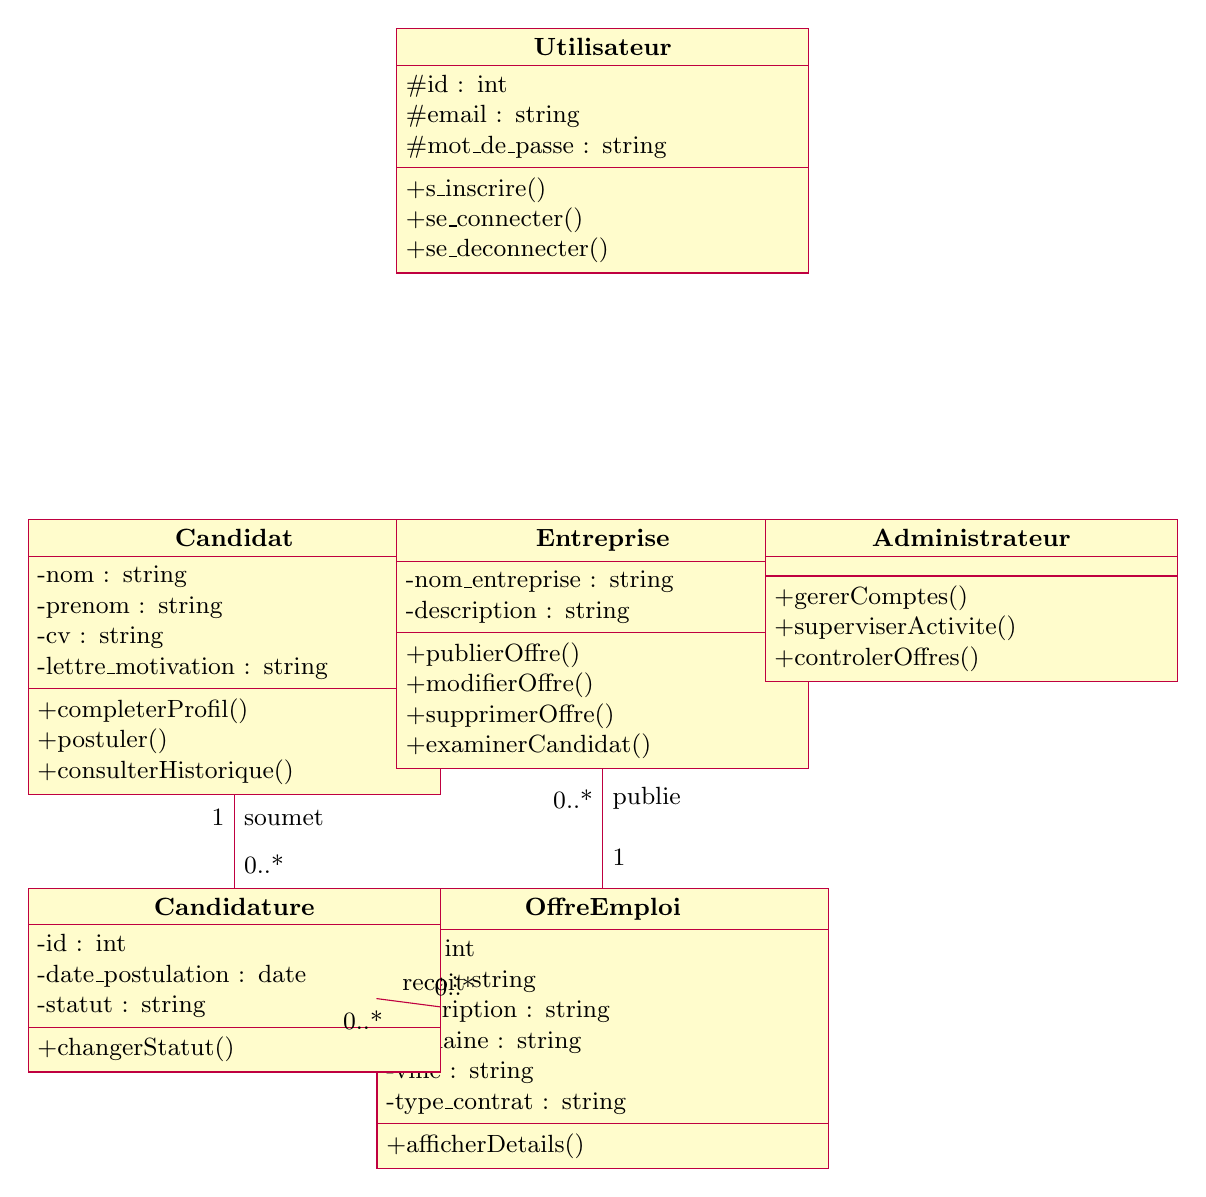
\begin{tikzpicture}[scale=0.78, every node/.style={font=\small}]
  % Utilisateur
  \begin{class}[text width=5cm]{Utilisateur}{0,8}
    \attribute{\#id : int}
    \attribute{\#email : string}
    \attribute{\#mot\_de\_passe : string}
    \operation{+s\_inscrire()}
    \operation{+se\_connecter()}
    \operation{+se\_deconnecter()}
  \end{class}

  % Candidat
  \begin{class}[text width=5cm]{Candidat}{-6,0}
    \attribute{-nom : string}
    \attribute{-prenom : string}
    \attribute{-cv : string}
    \attribute{-lettre\_motivation : string}
    \operation{+completerProfil()}
    \operation{+postuler()}
    \operation{+consulterHistorique()}
  \end{class}

  % Entreprise
  \begin{class}[text width=5cm]{Entreprise}{0,0}
    \attribute{-nom\_entreprise : string}
    \attribute{-description : string}
    \operation{+publierOffre()}
    \operation{+modifierOffre()}
    \operation{+supprimerOffre()}
    \operation{+examinerCandidat()}
  \end{class}

  % Administrateur
  \begin{class}[text width=5cm]{Administrateur}{6,0}
    \operation{+gererComptes()}
    \operation{+superviserActivite()}
    \operation{+controlerOffres()}
  \end{class}

  % OffreEmploi
  \begin{class}[text width=5.5cm]{OffreEmploi}{0,-6}
    \attribute{-id : int}
    \attribute{-titre : string}
    \attribute{-description : string}
    \attribute{-domaine : string}
    \attribute{-ville : string}
    \attribute{-type\_contrat : string}
    \operation{+afficherDetails()}
  \end{class}

  % Candidature
  \begin{class}[text width=5cm]{Candidature}{-6,-6}
    \attribute{-id : int}
    \attribute{-date\_postulation : date}
    \attribute{-statut : string}
    \operation{+changerStatut()}
  \end{class}

  % Héritages
  \inherit{Candidat}{Utilisateur}
  \inherit{Entreprise}{Utilisateur}
  \inherit{Administrateur}{Utilisateur}

  % Associations
  \association{Entreprise}{publie}{0..*}{OffreEmploi}{1}{}
  \association{Candidat}{soumet}{1}{Candidature}{0..*}{}
  \association{OffreEmploi}{recoit}{0..*}{Candidature}{0..*}{}
\end{tikzpicture}
\caption{Diagramme de classes de ManageraHub}
\end{figure}

% ─────────────────────────────────────────────────────────────────────────────
\section{Diagrammes de séquence}

\subsection{Présentation}

Les diagrammes de séquence modélisent les interactions dynamiques entre les objets du système au cours de l'exécution d'un scénario précis. Ils décrivent l'ordre chronologique des messages échangés entre les différentes entités participantes. Dans le cadre de ManageraHub, trois scénarios clés ont été modélisés~: le processus de postulation d'un candidat, le traitement d'une candidature par une entreprise, et le processus d'authentification.

\subsection{Diagramme de séquence~: Postulation d'un candidat}

Ce diagramme illustre le déroulement complet de l'action de postulation d'un candidat à une offre d'emploi. Le candidat commence par sélectionner une offre et cliquer sur le bouton «Postuler». Le système affiche alors le formulaire de candidature. Le candidat soumet ses documents (CV et lettre de motivation) via une requête HTTP POST. La vue \texttt{PostulerView} valide le formulaire Django~; si les données sont valides, la candidature est enregistrée en base de données avec le statut initial «En attente» et une notification est envoyée à l'entreprise concernée. Le candidat reçoit alors un message de confirmation. En cas d'erreur de validation, le formulaire est renvoyé avec les messages d'erreur appropriés.

\begin{figure}[H]
\centering
\begin{tikzpicture}[scale=0.75, every node/.style={font=\small}]
  % Lignes de vie
  \draw[thick] (0,0) -- (0,-10);
  \draw[thick] (3,0) -- (3,-10);
  \draw[thick] (6,0) -- (6,-10);
  \draw[thick] (9,0) -- (9,-10);
  \draw[thick] (12,0) -- (12,-10);

  % Têtes
  \node[draw, fill=darkplum!20, minimum width=2cm, minimum height=0.6cm] at (0,0.3) {Candidat};
  \node[draw, fill=periwinkle!30, minimum width=2cm, minimum height=0.6cm] at (3,0.3) {Template};
  \node[draw, fill=periwinkle!30, minimum width=2cm, minimum height=0.6cm] at (6,0.3) {PostulerView};
  \node[draw, fill=periwinkle!30, minimum width=2cm, minimum height=0.6cm] at (9,0.3) {Django Form};
  \node[draw, fill=darkplum!20, minimum width=2cm, minimum height=0.6cm] at (12,0.3) {MySQL};

  % Messages
  \draw[->] (0,-1) -- node[above, font=\tiny] {Clique Postuler} (3,-1);
  \draw[->] (3,-1.8) -- node[above, font=\tiny] {Affiche formulaire} (0,-1.8);
  \draw[->] (0,-2.6) -- node[above, font=\tiny] {POST /postuler/ (CV, Lettre)} (6,-2.6);
  \draw[->] (6,-3.4) -- node[above, font=\tiny] {is\_valid()} (9,-3.4);
  \draw[->] (9,-4.2) -- node[above, font=\tiny] {True} (6,-4.2);
  \draw[->] (6,-5) -- node[above, font=\tiny] {save() [statut=En attente]} (12,-5);
  \draw[->] (12,-5.8) -- node[above, font=\tiny] {Confirmation} (6,-5.8);
  \draw[->] (6,-6.6) -- node[above, font=\tiny] {messages.success()} (3,-6.6);
  \draw[->] (3,-7.4) -- node[above, font=\tiny] {«Candidature envoyée»} (0,-7.4);

  % Étiquettes axes
  \node[font=\tiny, gray] at (0,-10.3) {Candidat};
  \node[font=\tiny, gray] at (3,-10.3) {Template};
  \node[font=\tiny, gray] at (6,-10.3) {Vue};
  \node[font=\tiny, gray] at (9,-10.3) {Form};
  \node[font=\tiny, gray] at (12,-10.3) {MySQL};
\end{tikzpicture}
\caption{Diagramme de séquence~: Postulation d'un candidat}
\end{figure}

\subsection{Diagramme de séquence~: Traitement d'une candidature}

Ce diagramme modélise les interactions qui se produisent lorsqu'une entreprise traite une candidature reçue. L'entreprise accède à son tableau de bord et consulte la liste des candidatures pour une offre donnée. Le système interroge la base de données pour récupérer les candidatures filtrées selon le statut «En attente». Les profils des candidats (CV et lettres de motivation) sont affichés. L'entreprise prend ensuite l'une des trois décisions possibles~: accepter la candidature (statut mis à jour à «Accepté»), convoquer le candidat à un entretien (statut mis à jour à «Entretien») ou refuser la candidature (statut mis à jour à «Refusé»). Dans tous les cas, la base de données est mise à jour et une confirmation est affichée. Le candidat peut alors voir le nouveau statut depuis son propre espace.

\subsection{Diagramme de séquence~: Authentification}

Le scénario d'authentification décrit le processus de connexion d'un utilisateur. L'utilisateur saisit son adresse email et son mot de passe sur la page de connexion et soumet le formulaire. Le système vérifie que les données transmises correspondent à un compte existant en base de données. Si la correspondance est confirmée, une session est créée et l'utilisateur est redirigé vers son tableau de bord correspondant à son rôle (candidat, entreprise ou administrateur). En cas d'échec, un message d'erreur est affiché et l'utilisateur est invité à réessayer.

% ─────────────────────────────────────────────────────────────────────────────
\section{Modélisation de la base de données}

\subsection{Présentation du schéma relationnel}

La base de données de ManageraHub est conçue selon le modèle relationnel et est implémentée avec MySQL. Elle constitue le socle de persistance de l'ensemble des données manipulées par la plateforme. Le schéma a été élaboré à partir du diagramme de classes présenté précédemment, en respectant les règles de normalisation jusqu'à la troisième forme normale (3NF) afin d'éviter les redondances et de garantir l'intégrité des données.

\subsection{Description des tables principales}

\begin{table}[H]
\centering
\caption{Structure de la table \texttt{utilisateur}}
\begin{tabularx}{\textwidth}{llXl}
\toprule
\textbf{Champ} & \textbf{Type} & \textbf{Description} & \textbf{Contrainte} \\
\midrule
id & INT & Identifiant unique & PK, AUTO\_INCREMENT \\
email & VARCHAR(255) & Adresse email de connexion & UNIQUE, NOT NULL \\
mot\_de\_passe & VARCHAR(255) & Mot de passe hashé & NOT NULL \\
role & ENUM & Type d'utilisateur & NOT NULL \\
date\_creation & DATETIME & Date d'inscription & NOT NULL \\
\bottomrule
\end{tabularx}
\end{table}

\begin{table}[H]
\centering
\caption{Structure de la table \texttt{offre\_emploi}}
\begin{tabularx}{\textwidth}{llXl}
\toprule
\textbf{Champ} & \textbf{Type} & \textbf{Description} & \textbf{Contrainte} \\
\midrule
id & INT & Identifiant unique & PK, AUTO\_INCREMENT \\
entreprise\_id & INT & Référence à l'entreprise & FK \\
titre & VARCHAR(255) & Intitulé du poste & NOT NULL \\
description & TEXT & Description détaillée & NOT NULL \\
domaine & VARCHAR(100) & Secteur d'activité & NOT NULL \\
ville & VARCHAR(100) & Localisation du poste & NOT NULL \\
type\_contrat & VARCHAR(50) & CDI, CDD, Stage, etc. & NOT NULL \\
date\_publication & DATE & Date de mise en ligne & NOT NULL \\
\bottomrule
\end{tabularx}
\end{table}

\begin{table}[H]
\centering
\caption{Structure de la table \texttt{candidature}}
\begin{tabularx}{\textwidth}{llXl}
\toprule
\textbf{Champ} & \textbf{Type} & \textbf{Description} & \textbf{Contrainte} \\
\midrule
id & INT & Identifiant unique & PK, AUTO\_INCREMENT \\
candidat\_id & INT & Référence au candidat & FK \\
offre\_id & INT & Référence à l'offre & FK \\
date\_postulation & DATE & Date de soumission & NOT NULL \\
statut & ENUM & En attente / Accepté / Refusé / Entretien & NOT NULL \\
cv\_path & VARCHAR(500) & Chemin vers le CV & NOT NULL \\
lettre\_path & VARCHAR(500) & Chemin vers la lettre & -- \\
\bottomrule
\end{tabularx}
\end{table}

\section*{Conclusion}
\addcontentsline{toc}{section}{Conclusion du chapitre}

Ce second chapitre a présenté la conception détaillée de la plateforme ManageraHub à travers une série de modèles UML complémentaires. Le diagramme de cas d'utilisation a permis de clarifier les interactions entre les acteurs et le système. Le diagramme de classes a formalisé la structure statique du modèle de données, tandis que les diagrammes de séquence ont illustré les comportements dynamiques des scénarios clés. La modélisation de la base de données a enfin traduit ces abstractions en une structure de stockage concrète et cohérente. Ces éléments de conception constituent le guide de référence pour l'implémentation présentée dans le chapitre suivant.

% ═══════════════════════════════════════════════════════════════════════════════
%  CHAPITRE 3 : RÉALISATION
% ═══════════════════════════════════════════════════════════════════════════════
\chapter{Réalisation et Présentation de la Plateforme}

\section*{Introduction}
\addcontentsline{toc}{section}{Introduction}

Ce troisième et dernier chapitre présente les réalisations concrètes du projet ManageraHub. Après avoir défini le contexte et conçu le système dans les chapitres précédents, il s'agit maintenant d'exposer les différentes interfaces développées et de décrire les fonctionnalités implémentées. Ce chapitre met en valeur le travail de développement accompli et permet d'évaluer la correspondance entre les besoins exprimés et la solution effectivement réalisée.

% ─────────────────────────────────────────────────────────────────────────────
\section{Environnement de développement}

\subsection{Configuration de l'environnement}

Le développement de ManageraHub a été réalisé dans un environnement technique soigneusement configuré pour garantir la reproductibilité et la cohérence du processus de développement. Le système d'exploitation utilisé est Windows 11, avec Python 3.11 installé via un environnement virtuel dédié (venv). Le serveur de développement Django intégré a été utilisé pour les tests locaux, accessible à l'adresse \texttt{127.0.0.1:8000}. La base de données MySQL a été gérée localement, avec phpMyAdmin comme interface d'administration visuelle.

\subsection{Organisation du projet Django}

Le projet Django a été structuré selon les bonnes pratiques recommandées par la communauté Django. Le dossier principal du projet contient les fichiers de configuration (\texttt{settings.py}, \texttt{urls.py}). Plusieurs applications Django ont été créées pour organiser le code selon les domaines fonctionnels~: une application \texttt{accounts} gérant l'authentification et les profils, une application \texttt{offers} gérant les offres d'emploi, et une application \texttt{applications} gérant les candidatures. Les fichiers statiques (CSS, JavaScript, images) et les templates HTML sont organisés dans des répertoires dédiés.

\subsection{Outils de développement utilisés}

L'ensemble du développement a été réalisé avec Visual Studio Code comme éditeur de code principal, enrichi d'extensions dédiées au développement Python et Django. Git a été utilisé pour le contrôle de version, avec un dépôt hébergé sur GitHub facilitant la collaboration entre les deux membres de l'équipe. Les tests unitaires ont été réalisés avec le framework de tests intégré à Django.

% ─────────────────────────────────────────────────────────────────────────────
\section{Page d'accueil et navigation}

\subsection{Page d'accueil publique}

La page d'accueil constitue la vitrine de la plateforme ManageraHub. Elle s'adresse aussi bien aux visiteurs non encore inscrits qu'aux utilisateurs connectés cherchant à naviguer rapidement vers leur espace. Elle présente de manière claire et visuelle la proposition de valeur de la plateforme, avec un slogan accrocheur et deux appels à l'action principaux dirigeant respectivement les candidats et les entreprises vers leurs espaces dédiés.

La partie supérieure de la page intègre une barre de navigation fixe proposant les liens vers les différentes sections du site. Un bandeau héros (hero banner) occupe la majeure partie de l'écran en mode plein page, avec une photographie d'ambiance professionnelle en arrière-plan sur laquelle le nom de la plateforme et le slogan sont affichés en grand format. Deux boutons d'appel à l'action («Explore Opportunities» et «For Companies») permettent aux visiteurs d'accéder rapidement à la section qui les concerne.

\subsection{Section des services}

Immédiatement en dessous du bandeau principal, une section dédiée aux services présente les deux propositions de valeur clés de ManageraHub. D'un côté, la section destinée aux candidats met en avant la possibilité de créer un profil, de téléverser un CV et de postuler en ligne. De l'autre, la section entreprise souligne les avantages liés à la publication d'offres et à la gestion centralisée des candidatures. Chaque section dispose d'un bouton d'inscription permettant à l'utilisateur de démarrer immédiatement son parcours sur la plateforme.

% ─────────────────────────────────────────────────────────────────────────────
\section{Authentification et gestion des comptes}

\subsection{Page de connexion}

La page de connexion de ManageraHub adopte une mise en page en deux colonnes. La colonne de gauche affiche une image de fond plein écran avec un message d'accueil et une accroche motivante. La colonne de droite, sur fond sombre semi-transparent, contient le formulaire de connexion. Ce formulaire propose d'abord une sélection du type de compte (Candidat ou Entreprise) via des boutons exclusifs, puis les champs email et mot de passe. Des liens vers les formulaires d'inscription et une option de récupération de mot de passe complètent l'interface. Des boutons permettent également une connexion via les comptes Google ou GitHub, exploitant les mécanismes d'authentification OAuth.

\subsection{Formulaire d'inscription candidat}

Le formulaire d'inscription des candidats suit la même structure en deux colonnes. La partie gauche présente la plateforme avec un argumentaire destiné aux candidats, tandis que la partie droite contient le formulaire structuré en plusieurs sections. Une première section collecte les informations personnelles (prénom, nom, email, téléphone, pays, ville, date de naissance). Une section dédiée à la sécurité du compte recueille le mot de passe et sa confirmation, avec des indications sur les critères de complexité requis (minimum 8 caractères, incluant lettres, chiffres et symboles). Une section relative aux conditions générales propose deux cases à cocher, l'une obligatoire pour l'acceptation des termes d'utilisation, l'autre optionnelle pour l'abonnement aux actualités de la plateforme.

\subsection{Formulaire d'inscription entreprise}

Le formulaire d'inscription entreprise est conçu de manière similaire à celui des candidats, avec des adaptations spécifiques au contexte professionnel. Les informations collectées incluent le nom de l'entreprise, son secteur d'activité, sa taille, l'adresse email professionnelle et le numéro de téléphone. Les conditions d'utilisation présentées à l'entreprise comprennent trois cases à cocher~: une confirmation de l'autorisation à représenter l'entité juridique, une certification de l'exactitude des informations fournies, et une option d'abonnement aux actualités de la plateforme. Le bouton de validation final lance la création du compte entreprise après vérification de l'ensemble des champs requis.

% ─────────────────────────────────────────────────────────────────────────────
\section{Espace candidat}

\subsection{Tableau de bord du candidat}

Après connexion, le candidat accède à son tableau de bord personnel. Cet espace centralisé lui offre une vue d'ensemble de son activité sur la plateforme~: le nombre de candidatures soumises, le nombre de candidatures en attente, les candidatures acceptées et celles qui ont conduit à une invitation à un entretien. Des indicateurs visuels permettent d'identifier rapidement l'état de chaque démarche. Un menu latéral donne accès aux différentes sections de l'espace candidat~: son profil, ses candidatures, les offres disponibles et les paramètres de son compte.

\subsection{Gestion du profil candidat}

La section profil permet au candidat de compléter et de mettre à jour l'ensemble de ses informations personnelles et professionnelles. Il peut y renseigner son parcours académique, ses expériences professionnelles, ses compétences et ses langues maîtrisées. Un module de téléversement de fichiers lui permet d'importer son CV au format PDF ou Word. La page de profil affiche également une indication de complétude du profil, encourageant le candidat à fournir un maximum d'informations pour maximiser ses chances.

\subsection{Recherche et consultation des offres}

Le moteur de recherche d'offres permet au candidat de trouver les annonces correspondant à son profil. Il dispose de plusieurs critères de filtrage cumulables~: le domaine d'activité, la ville, le type de contrat, et une recherche textuelle libre sur le titre ou la description de l'offre. Les résultats sont affichés sous forme de cartes synthétiques présentant les informations essentielles de chaque annonce. En cliquant sur une offre, le candidat accède à la page de détail qui présente l'ensemble des informations~: description complète du poste, profil recherché, conditions de travail et coordonnées de l'entreprise.

\subsection{Soumission et suivi des candidatures}

Depuis la page de détail d'une offre, le candidat peut initier sa candidature en cliquant sur le bouton dédié. Un formulaire lui demande de confirmer les documents à transmettre (CV et éventuellement une lettre de motivation spécifique à cette offre) et de valider sa soumission. Une fois la candidature envoyée, elle apparaît dans la section «Mes candidatures» avec le statut «En attente». Cette section lui permet de consulter l'historique complet de ses démarches et de suivre les évolutions de statut au fil du temps.

% ─────────────────────────────────────────────────────────────────────────────
\section{Espace entreprise}

\subsection{Tableau de bord de l'entreprise}

L'espace entreprise est organisé autour d'un tableau de bord centralisé offrant une vision globale de l'activité de recrutement. Des indicateurs clés présentent le nombre total d'offres publiées, le nombre de candidatures reçues en attente de traitement, et le nombre de recrutements finalisés. Un accès rapide aux offres récentes et aux nouvelles candidatures permet à l'entreprise de prioriser ses actions.

\subsection{Gestion des offres d'emploi}

La section de gestion des offres permet à l'entreprise de créer de nouvelles annonces via un formulaire structuré collectant l'ensemble des informations nécessaires~: intitulé du poste, description détaillée, compétences requises, type de contrat, localisation et date limite de dépôt des candidatures. L'entreprise peut également consulter la liste de ses offres actives, modifier les informations d'une annonce existante ou la désactiver si le poste a été pourvu.

\subsection{Gestion des candidatures reçues}

Pour chaque offre, l'entreprise dispose d'une vue dédiée listant l'ensemble des candidatures reçues. Chaque entrée affiche les informations synthétiques du candidat et son statut courant. En cliquant sur une candidature, le recruteur accède au profil complet du candidat, peut télécharger son CV et consulter sa lettre de motivation. Trois boutons d'action lui permettent de prendre sa décision~: «Accepter» (statut mis à jour à Accepté), «Convoquer à un entretien» (statut Entretien) ou «Refuser» (statut Refusé). Chaque action déclenche automatiquement une mise à jour visible par le candidat dans son propre espace.

% ─────────────────────────────────────────────────────────────────────────────
\section{Interface d'administration}

\subsection{Tableau de bord administrateur}

L'interface d'administration offre à l'administrateur une vue d'ensemble complète de la plateforme. Des statistiques globales présentent le nombre total d'utilisateurs inscrits (candidats et entreprises), le nombre d'offres actives et le volume total de candidatures traitées. Des graphiques d'évolution permettent de suivre la croissance de la plateforme dans le temps.

\subsection{Gestion des utilisateurs}

L'administrateur dispose d'un outil de gestion des comptes lui permettant de consulter la liste complète des utilisateurs, de rechercher un compte spécifique, de consulter les détails d'un profil, de suspendre temporairement un compte ou de le supprimer définitivement. Cette fonctionnalité lui permet d'intervenir rapidement en cas de signalement ou de comportement abusif sur la plateforme.

\subsection{Supervision des offres}

La section de supervision des offres liste l'ensemble des annonces publiées sur la plateforme, quel que soit l'entreprise émettrice. L'administrateur peut consulter le contenu de chaque offre et la supprimer si elle ne respecte pas les règles d'utilisation de la plateforme. Il dispose également d'un accès aux statistiques de consultation de chaque offre, lui permettant d'identifier les annonces les plus populaires.

% ─────────────────────────────────────────────────────────────────────────────
\section{Charte graphique et ergonomie}

\subsection{Identité visuelle}

L'identité visuelle de ManageraHub repose sur une palette de couleurs soigneusement sélectionnée pour transmettre les valeurs de professionnalisme, de confiance et de modernité qui fondent la proposition de la plateforme. La couleur principale, Dark Plum (\texttt{\#4F0C28}), un bordeaux profond, est utilisée pour les éléments structurants de l'interface~: les titres, les boutons primaires, les bordures d'accent et les éléments de navigation. Le Periwinkle (\texttt{\#C5D2F8}), un bleu-lavande clair, apporte de la fraîcheur et de la modernité dans les zones secondaires. Le blanc cassé (\texttt{\#F1FAEE}) constitue la couleur de fond principale, garantissant une lisibilité optimale et une atmosphère apaisante.

\subsection{Typographie}

Deux familles typographiques ont été sélectionnées pour assurer la cohérence visuelle de l'interface. Poppins, une police sans-sérif géométrique moderne aux proportions équilibrées, est utilisée pour les titres et les éléments d'accroche. Inter, reconnue pour son excellente lisibilité à toutes les tailles, est privilégiée pour le corps du texte et les éléments informatifs. Cette combinaison assure une hiérarchie visuelle claire et une lecture confortable sur tous les types d'écrans.

\subsection{Principes d'ergonomie}

La conception ergonomique de ManageraHub a été guidée par plusieurs principes fondamentaux. La clarté de l'interface est assurée par une utilisation généreuse des espaces blancs, évitant la surcharge visuelle. La hiérarchie de l'information est respectée par une utilisation cohérente des tailles de police et des niveaux de contraste. La cohérence des interactions est garantie par l'utilisation des mêmes composants d'interface (boutons, formulaires, cartes) dans l'ensemble de la plateforme. La réactivité du design assure une expérience optimale aussi bien sur les écrans d'ordinateur que sur les tablettes.

\section*{Conclusion}
\addcontentsline{toc}{section}{Conclusion du chapitre}

Ce troisième chapitre a présenté les réalisations concrètes de la plateforme ManageraHub. Les différentes interfaces développées reflètent fidèlement les besoins identifiés dans le premier chapitre et la conception définie dans le second. La plateforme offre un parcours utilisateur fluide et cohérent pour chacune des trois catégories d'acteurs, depuis l'inscription jusqu'à la finalisation du processus de recrutement. La charte graphique adoptée renforce l'identité professionnelle de la solution et contribue à une expérience utilisateur de qualité.

% ─── Conclusion générale ─────────────────────────────────────────────────────
\chapter*{Conclusion Générale et Perspectives}
\addcontentsline{toc}{chapter}{Conclusion Générale et Perspectives}
\markboth{Conclusion Générale et Perspectives}{}

\section*{Bilan du projet}

Le projet ManageraHub a permis de concevoir et de développer une plateforme web de recrutement complète, répondant aux besoins identifiés aussi bien du côté des candidats que des entreprises. Tout au long de ce travail, nous avons mis en pratique les compétences acquises au cours de notre formation en Ingénierie Informatique et Réseaux à l'EMSI, en couvrant l'ensemble du cycle de développement logiciel, de l'analyse des besoins à la réalisation.

Sur le plan technique, le projet a permis d'approfondir notre maîtrise du framework Django et de son ORM, de consolider nos connaissances en modélisation de bases de données relationnelles MySQL, et de développer nos compétences en conception d'interfaces web modernes et ergonomiques. La gestion collaborative du code source via GitHub a également constitué une expérience formatrice dans le domaine du travail d'équipe appliqué au développement logiciel.

Sur le plan méthodologique, la rédaction du cahier des charges, l'élaboration des diagrammes UML et la structuration du rapport nous ont initiés aux pratiques professionnelles de la gestion de projet informatique, qui constituent des compétences essentielles dans notre future vie professionnelle.

\section*{Perspectives d'évolution}

Bien que la version actuelle de ManageraHub satisfasse aux objectifs fonctionnels définis dans le cahier des charges, plusieurs axes d'évolution peuvent être envisagés pour enrichir la plateforme dans ses prochaines versions.

L'intégration d'un \textbf{système de recommandation basé sur l'intelligence artificielle} constitue la piste la plus prometteuse. En analysant le profil d'un candidat (compétences, expériences, préférences), un algorithme de recommandation pourrait suggérer automatiquement les offres les plus pertinentes, améliorant ainsi l'expérience de recherche. Symétriquement, les entreprises pourraient bénéficier de suggestions de profils correspondant à leurs offres.

Le développement d'une \textbf{application mobile native} (iOS et Android) permettrait d'élargir l'accessibilité de la plateforme et de toucher un public plus large, notamment les jeunes actifs habitués à gérer leur vie professionnelle depuis leur smartphone.

L'ajout d'un \textbf{système de messagerie interne} permettrait aux entreprises et aux candidats de communiquer directement sur la plateforme, sans avoir recours à des canaux externes. Cela renforcerait la centralisation du processus et améliorerait la traçabilité des échanges.

L'intégration de \textbf{fonctionnalités d'analyse et de reporting} permettrait aux entreprises de disposer de tableaux de bord avancés avec des métriques détaillées sur leurs recrutements (taux de conversion, délai moyen de recrutement, sources des candidatures), facilitant ainsi l'optimisation de leurs stratégies de recrutement.

Enfin, la mise en conformité avec le \textbf{Règlement Général sur la Protection des Données (RGPD)} et les réglementations marocaines en matière de protection des données personnelles constitue une évolution obligatoire avant tout déploiement en environnement de production.

% ─── Références ──────────────────────────────────────────────────────────────
\chapter*{Références Bibliographiques}
\addcontentsline{toc}{chapter}{Références Bibliographiques}
\markboth{Références Bibliographiques}{}

\begin{enumerate}[leftmargin=*, label={[\arabic*]}]
  \item Django Software Foundation. \textit{Django Documentation}. \url{https://docs.djangoproject.com/}
  \item MySQL AB. \textit{MySQL 8.0 Reference Manual}. Oracle Corporation. \url{https://dev.mysql.com/doc/}
  \item Fowler, M. \textit{UML Distilled: A Brief Guide to the Standard Object Modeling Language}. 3rd ed. Addison-Wesley Professional, 2003.
  \item Gamma, E., Helm, R., Johnson, R., \& Vlissides, J. \textit{Design Patterns: Elements of Reusable Object-Oriented Software}. Addison-Wesley Professional, 1994.
  \item Lutz, M. \textit{Learning Python}. 5th ed. O'Reilly Media, 2013.
  \item Holovaty, A., \& Kaplan-Moss, J. \textit{The Definitive Guide to Django}. Apress, 2009.
  \item Nielsen, J. \textit{Usability Engineering}. Morgan Kaufmann Publishers, 1994.
  \item W3Schools. \textit{HTML, CSS, JavaScript Tutorials}. \url{https://www.w3schools.com/}
  \item GitHub Documentation. \textit{Getting Started with GitHub}. \url{https://docs.github.com/}
  \item Rekrute.com. \textit{Plateforme de recrutement au Maroc}. \url{https://www.rekrute.com/}
\end{enumerate}

\end{document}
